\documentclass[11pt]{report} % Select font size and documentclass
\usepackage[utf8]{inputenc} % Enables LaTeX to handle Unicode Characters directly 
%\usepackage[utf8x]{inputenc}
\usepackage[table]{xcolor} % For table cells color
\usepackage{mathptmx} % Used to change the default font in math mode
\usepackage{amsmath} % To write mathematical equation
\usepackage{graphicx} % Used to include external graphics
\usepackage{animate} % for animation
\usepackage{subcaption} % To present multiple related images or tables within a single figure
\usepackage{booktabs} % to creat high quality tables
\usepackage{circuitikz} % to draw electrical circuit
\usepackage{siunitx} % for si unit
\usepackage{tikz} % to draaw flow chart
\usetikzlibrary{shapes.geometric, arrows} % for flow chart
\usepackage{float} % enhanced control over the placement of floating element
\usepackage{enumerate} % to customize the appereance of lists
\usepackage{enumitem}
\usepackage[colorlinks,linkcolor=black, citecolor=blue, urlcolor=blue]{hyperref} % to enable the creation of hyperlinks
\usepackage{geometry} % for margin specification
\geometry{left=3.5cm,right=2.5cm,top=2.5cm,bottom=2.5cm} % set margin
\usepackage{setspace} % set space between line
\onehalfspacing
% \usepackage{fontspec} % to utilize fonts installed on system directly
% \setmainfont{Times New Roman}
\usepackage{titlesec}
\usepackage{fancyhdr} % to customize header and footer
\usepackage{lipsum} % to generate dummy text
\usepackage{lastpage} % page numbering
\usepackage{etoolbox} % provides tools for modifying and patching LaTeX commands. 
\usepackage{cite} % of citations and bibliographies in LaTeX.
\usepackage{pifont} % for special symbol uses
% Example: \ding{number}
\usepackage{eso-pic}

%%%%%%%%%%%%% Split document into multiple column %%%%%%%%%%%%
\usepackage{multicol}
\setlength{\columnsep}{1cm}
\setlength{\columnseprule}{1pt}
\def\columnseprulecolor{\color{black}}

%%%%%%%%%%%%%%%%%% Boxed Text %%%%%%%%%%%


%%%%%%%%%%%%%%%%%%%%%%% Coding Style %%%%%%%%%%%%%%%%%%%%%%%%%
\usepackage{listings}
\usepackage{xcolor}

%New colors defined below
\definecolor{codegreen}{rgb}{0,0.6,0}
\definecolor{codegray}{rgb}{0.5,0.5,0.5}
\definecolor{codepurple}{rgb}{0.58,0,0.82}
\definecolor{backcolour}{rgb}{0.95,0.95,0.92}

%Code listing style named "mystyle"
\lstdefinestyle{mystyle}{
  backgroundcolor=\color{backcolour}, commentstyle=\color{codegreen},
  keywordstyle=\color{magenta},
%  numberstyle=\tiny\color{codegray},
  numberstyle=false,
  stringstyle=\color{codepurple},
%  basicstyle=\ttfamily\small,
  basicstyle=\fontsize{10}{10}\selectfont\ttfamily,
  breakatwhitespace=false,         
  breaklines=true,                 
  captionpos=b,                    
  keepspaces=true,                 
%  numbers=left,                    
  numbersep=5pt,                  
  showspaces=false,                
  showstringspaces=false,
  showtabs=false,                  
  tabsize=4
}

\lstset{style=mystyle}


%%%%%%%%%%%%%%%%%%%%%%%%%%%%%%%%%%%%%%%%%%%

\usepackage{lmodern} % to control font-size
%% {\fontsize{font size}{base line strech} \selectfont}
%% {\fontsize{40}{48} \selectfont Dynamic} % syntex to control fontsize.

\usepackage{tabularx}
\usepackage{makecell}
\usepackage{multirow}
\usepackage{multicol}
\usepackage{hhline}
\usepackage{pgf-pie}
\usetikzlibrary{backgrounds}
\usepackage{courier}
\newcommand\tab[1][1cm]{\hspace*{#1}}
\newcommand{\head}[1]{\textnormal{\textbf{#1}}}
\newcommand{\HRule}{\rule{\linewidth}{0.5mm}}

%%%%%%%%%%%% To Draw Figures %%%%%%%%%%%
\usepackage{tikz}
\usetikzlibrary{positioning}
\usepackage{hvlogos}

%%%%%%% Matrix %%%%%%%%%%%%
\usepackage{amsmath,blkarray,booktabs, bigstrut}


%------------ For Cover Page -----------------
\newcommand*{\plogo}{\fbox{$\mathcal{PL}$}} % Generic dummy publisher logo

\usepackage[utf8]{inputenc} % Required for inputting international characters
\usepackage[T1]{fontenc} % Output font encoding for international characters
\usepackage{stix} % Use the STIX fonts


\begin{document}

%----------------------------------------------------------------------------------------
%	                 TITLE PAGE
%----------------------------------------------------------------------------------------

	%%%%%%%%%%%%%%%%%%%%%%%%%%%%%%%%%%%%%%%%%
% Vertical Line Title Page
% LaTeX Template
% Version 2.0 (22/7/17)
%
% This template was downloaded from:
% http://www.LaTeXTemplates.com
%
% Original author:
% Peter Wilson (herries.press@earthlink.net) with modifications by:
% Vel (vel@latextemplates.com)
%
% License:
% CC BY-NC-SA 3.0 (http://creativecommons.org/licenses/by-nc-sa/3.0/)
% 
% This template can be used in one of two ways:
%
% 1) Content can be added at the end of this file just before the \end{document}
% to use this title page as the starting point for your document.
%
% 2) Alternatively, if you already have a document which you wish to add this
% title page to, copy everything between the \begin{document} and
% \end{document} and paste it where you would like the title page in your
% document. You will then need to insert the packages and document 
% configurations into your document carefully making sure you are not loading
% the same package twice and that there are no clashes.
%
%%%%%%%%%%%%%%%%%%%%%%%%%%%%%%%%%%%%%%%%%

%----------------------------------------------------------------------------------------
%	PACKAGES AND OTHER DOCUMENT CONFIGURATIONS
%----------------------------------------------------------------------------------------

\documentclass[a4paper, 11pt]{book} % A4 paper size and default 11pt font size

\newcommand*{\plogo}{\fbox{$\mathcal{PL}$}} % Generic dummy publisher logo

\usepackage[utf8]{inputenc} % Required for inputting international characters
\usepackage[T1]{fontenc} % Output font encoding for international characters
\usepackage{stix} % Use the STIX fonts

\begin{document}

%----------------------------------------------------------------------------------------
%	TITLE PAGE
%----------------------------------------------------------------------------------------

\begin{titlepage} % Suppresses displaying the page number on the title page and the subsequent page counts as page 1
	
	\raggedleft % Right align the title page
	
	\rule{1pt}{\textheight} % Vertical line
	\hspace{0.05\textwidth} % Whitespace between the vertical line and title page text
	\parbox[b]{0.75\textwidth}{ % Paragraph box for holding the title page text, adjust the width to move the title page left or right on the page
		
		{\Huge\bfseries A Collection of \\[0.5\baselineskip] \LaTeX ~Templates}\\[2\baselineskip] % Title
		{\large\textit{A predictable subtitle}}\\[4\baselineskip] % Subtitle or further description
		{\Large\textsc{gordon freeman}} % Author name, lower case for consistent small caps
		
		\vspace{0.5\textheight} % Whitespace between the title block and the publisher
		
		{\noindent The Publisher~~\plogo}\\[\baselineskip] % Publisher and logo
	}

\end{titlepage}

%----------------------------------------------------------------------------------------

\end{document}


	
	%%%%%%%%%%%%%%%%%%% Table of Contents  %%%%%%%%%%%%%%%%
	\tableofcontents
	\pagenumbering{\roman}	
	
	%%%%%%%%%%%%%%%%%% Page Numbering Style %%%%%%%%%%%%%%
	\pagenumbering{arabic}
	\patchcmd{\chapter}{\thispagestyle{plain}}{\thispagestyle{fancy}}{}{}
	\fancypagestyle{main}{
    	\fancyhf{} % clear all header and footer fields
    	\renewcommand{\headrulewidth}{0pt} % remove header rule
    	\renewcommand{\footrulewidth}{1pt} % set footerr rule
    	\fancyfoot[L]{
%    		\href{mailto:aongcho880@gmail.com}{\underline{Aong Cho Marma}}\\
    		\fontsize{10}{10}\selectfont \leftmark
    	} % chapter name at left footer
    	\fancyfoot[R]{Page \thepage\ of \pageref{LastPage}} % page number at center footer
	}
	
	\pagestyle{main} % set the main page style
	\setcounter{page}{1}
	% Define style for equation numbers
	\renewcommand{\theequation}{\arabic{chapter}.\arabic{equation}}
	
	%%%%%%%%%%%%%%%%%%%%%%%%%%%%%%%%%%%%%%%%%%%%%
	
	%%%%%%%%%%%%%%% Chapters %%%%%%%%%%%%%%%%%%%%
	
	\chapter{Displaying Data from Multiple Tables}

\section{\textbf{Practice 6}}

%--------------------------------------
\subsubsection*{Problem 01}
\addcontentsline{toc}{subsection}{Problem 01}
Write a query for the HR department to produce the addresses of all the departments. Use the LOCATIONS and COUNTRIES tables. Show the location ID, street address, city, state or province, and country in the output. Use a NATURAL JOIN to produce the results.

\begin{frame}

\AddToShipoutPictureFG*{ % Add figure to foreground of current page
  \put(\LenToUnit{5.5cm},\LenToUnit{5cm}){% Adjust the coordinates as needed
    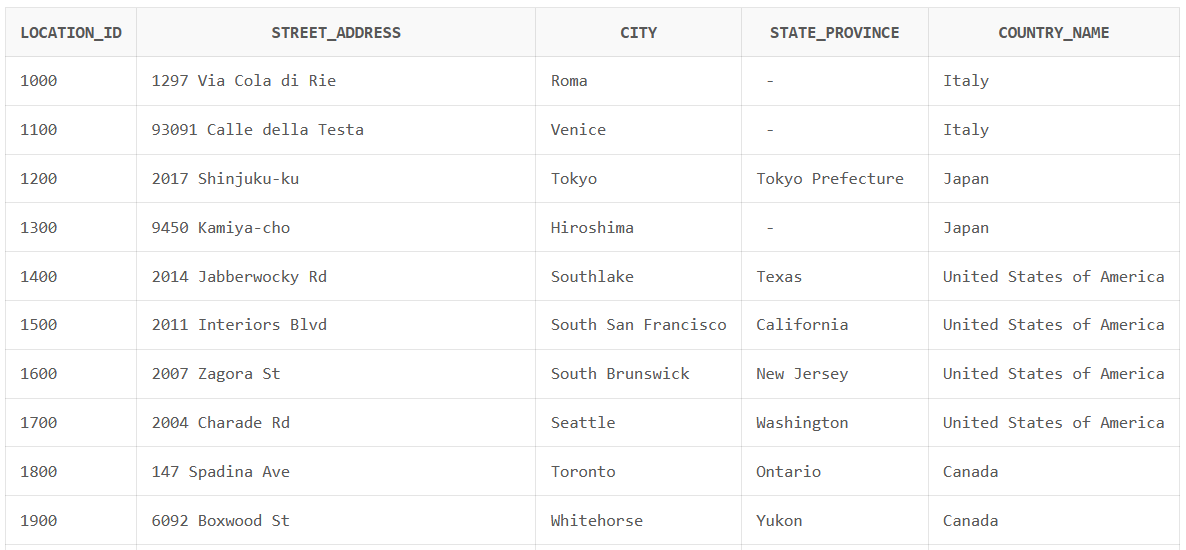
\includegraphics[width=13cm]{Figs/fig_601.png}
  }
}

\lstset{
  basicstyle=\fontsize{10}{12}\selectfont\ttfamily
}

\begin{lstlisting}[language=SQL]
SELECT 	location_id, street_address, city, 
    	state_province, country_name
FROM	hr.locations
NATURAL JOIN hr.countries;
\end{lstlisting}
\textbf{Output: }
\end{frame}


%--------------------------------------
\newpage
\subsubsection*{Problem 02}
\addcontentsline{toc}{subsection}{Problem 02}
The HR department needs a report of all employees. Write a query to display the last name, department number, and department name for all the employees.

\begin{frame}

\AddToShipoutPictureFG*{ % Add figure to foreground of current page
  \put(\LenToUnit{5.5cm},\LenToUnit{14.5cm}){% Adjust the coordinates as needed
    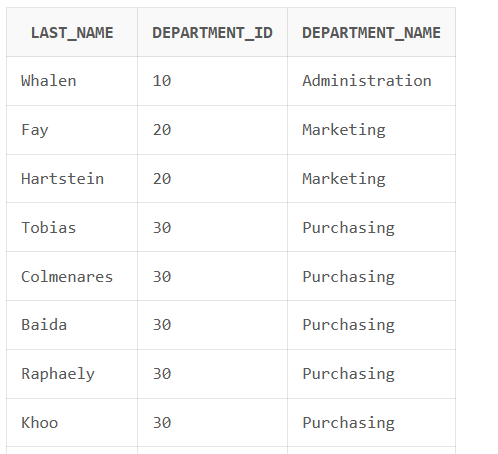
\includegraphics[width=7cm]{Figs/fig_602.png}
  }
}

\lstset{
  basicstyle=\fontsize{10}{12}\selectfont\ttfamily
}

\begin{lstlisting}[language=SQL]
SELECT 	last_name, department_id, department_name
FROM	hr.employees
JOIN	hr.departments USING (department_id);
\end{lstlisting}
\textbf{Output: }
\end{frame}


%--------------------------------------
\vspace{6.5cm}
\subsubsection*{Problem 03}
\addcontentsline{toc}{subsection}{Problem 03}
The HR department needs a report of all employees. Write a query to display the last name, department number, and department name for all the employees.

\begin{frame}

\AddToShipoutPictureFG*{ % Add figure to foreground of current page
  \put(\LenToUnit{5.5cm},\LenToUnit{3cm}){% Adjust the coordinates as needed
    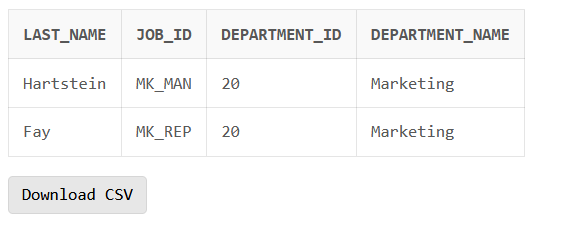
\includegraphics[width=10cm]{Figs/fig_603.png}
  }
}

\lstset{
  basicstyle=\fontsize{10}{12}\selectfont\ttfamily
}

\begin{lstlisting}[language=SQL]
SELECT 	last_name, job_id, department_id, department_name
FROM 	hr.employees
JOIN	hr.departments USING (department_id)
JOIN	hr.locations USING (location_id)
WHERE	city = 'Toronto';
\end{lstlisting}
\textbf{Output: }
\end{frame}

%-----------------------------
\newpage
\subsubsection*{Problem 04}
\addcontentsline{toc}{subsection}{Problem 04}
Create a report to display employees last name and employee number along with their managers last name and manager number. Label the columns Employee, Emp\#, Manager, and Mgr\#, respectively. Run the query.

\begin{frame}

\AddToShipoutPictureFG*{ % Add figure to foreground of current page
  \put(\LenToUnit{13cm},\LenToUnit{15.3cm}){% Adjust the coordinates as needed
    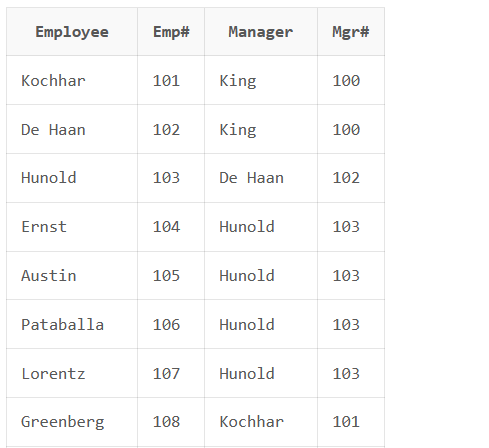
\includegraphics[width=7cm]{Figs/fig_604.png}
  }
}

\lstset{
  basicstyle=\fontsize{10}{12}\selectfont\ttfamily
}

\begin{lstlisting}[language=SQL]
SELECT 	e.last_name AS "Employee",
		e.employee_id AS "Emp#",
		m.last_name AS "Manager",
		m.employee_id AS "Mgr#"
    
FROM	hr.employees e
JOIN	hr.employees m 
		ON (e.manager_id = m.employee_id)
ORDER BY	e.employee_id;
\end{lstlisting}
\textbf{Output: }
\end{frame}

%----------------------------
\vspace{0.5cm}
\subsubsection*{Problem 05}
\addcontentsline{toc}{subsection}{Problem 05}
Modify lab\_06\_04.sql to display all employees including King, who has no manager. Order the results by the employee number. Save your SQL statement as lab\_06\_05.sql. Run the query in lab\_06\_05.sql.

\begin{frame}

\AddToShipoutPictureFG*{ % Add figure to foreground of current page
  \put(\LenToUnit{5.5cm},\LenToUnit{2.3cm}){% Adjust the coordinates as needed
    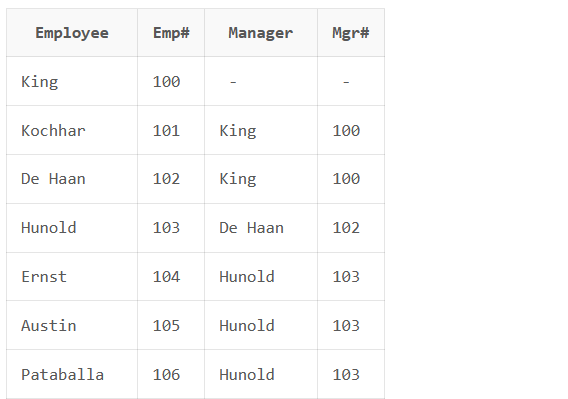
\includegraphics[width=9cm]{Figs/fig_605.png}
  }
}

\lstset{
  basicstyle=\fontsize{10}{12}\selectfont\ttfamily
}

\begin{lstlisting}[language=SQL]
SELECT e.last_name AS "Employee",
       e.employee_id AS "Emp#",
       m.last_name AS "Manager",
       m.employee_id AS "Mgr#"
FROM   hr.employees e
LEFT JOIN hr.employees m ON (e.manager_id = m.employee_id)
ORDER BY e.employee_id;
\end{lstlisting}
\textbf{Output: }
\end{frame}


%-----------------------------
\newpage
\subsubsection*{Problem 06}
\addcontentsline{toc}{subsection}{Problem 06}
Create a report for the HR department that displays employee last names, department numbers, and all the employees who work in the same department as a given employee. Give each column an appropriate label. Save the script to a file named lab\_06\_06.sql.

\begin{frame}

\AddToShipoutPictureFG*{ % Add figure to foreground of current page
  \put(\LenToUnit{13cm},\LenToUnit{12.5cm}){% Adjust the coordinates as needed
    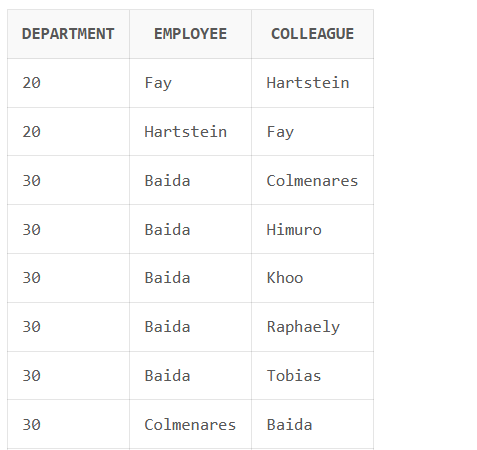
\includegraphics[width=7cm]{Figs/fig_606.png}
  }
}

\lstset{
  basicstyle=\fontsize{10}{12}\selectfont\ttfamily
}

\begin{lstlisting}[language=SQL]
SELECT 	e.department_id AS department,
       	e.last_name AS employee,
       	c.last_name AS colleague
FROM 	hr.employees e
JOIN 	hr.employees c ON (e.department_id = c.department_id)
WHERE 	e.employee_id <> c.employee_id
ORDER BY department, employee, colleague;
\end{lstlisting}
\textbf{Output: }
\end{frame}

%---------------------------
\vspace{4cm}
\subsubsection*{Problem 08}
\addcontentsline{toc}{subsection}{Problem 08}
The HR department wants to determine the names of all the employees who were hired after Davies. Create a query to display the name and hire date of any employee hired after employee Davies.
\begin{frame}

\AddToShipoutPictureFG*{ % Add figure to foreground of current page
  \put(\LenToUnit{5.5cm},\LenToUnit{2.3cm}){% Adjust the coordinates as needed
    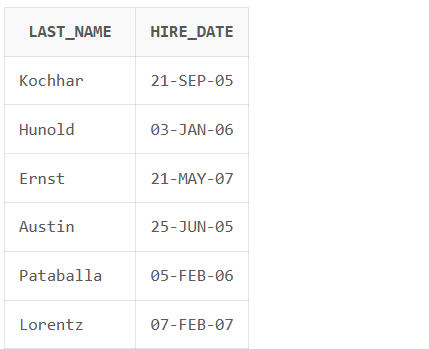
\includegraphics[width=7cm]{Figs/fig_608.png}
  }
}

\lstset{
  basicstyle=\fontsize{10}{12}\selectfont\ttfamily
}

\begin{lstlisting}[language=SQL]
SELECT 	e.last_name,
       	TO_CHAR (e.hire_date, 'DD-MON-YY') hire_date
FROM 	hr.employees e
JOIN 	hr.employees davies ON (davies.last_name = 'Davies')
WHERE 	davies.hire_date < e.hire_date;
\end{lstlisting}
\textbf{Output: }
\end{frame}


%-----------------------------
\newpage
\subsubsection*{Problem 09}
\addcontentsline{toc}{subsection}{Problem 09}
The HR department needs to find the names and hire dates of all the employees who were hired before their managers, along with their managers names and hire dates. Save the script to a file named lab\_06\_09.sql.

\begin{frame}

\AddToShipoutPictureFG*{ % Add figure to foreground of current page
  \put(\LenToUnit{5.5cm},\LenToUnit{10.2cm}){% Adjust the coordinates as needed
    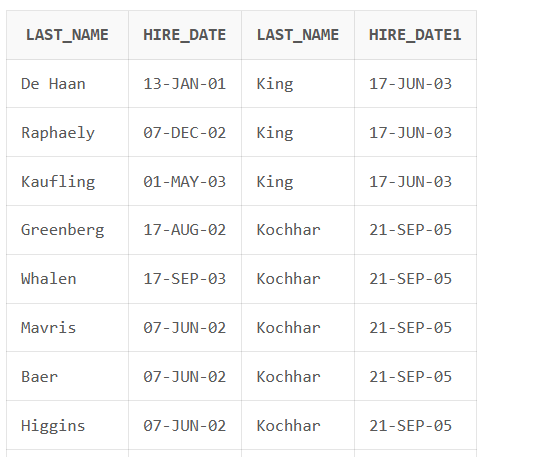
\includegraphics[width=9cm]{Figs/fig_609.png}
  }
}

\lstset{
  basicstyle=\fontsize{10}{12}\selectfont\ttfamily
}

\begin{lstlisting}[language=SQL]
SELECT 	e.last_name,
       	TO_CHAR (e.hire_date, 'DD-MON-YY') hire_date,
       	m.last_name,
       	TO_CHAR (m.hire_date, 'DD-MON-YY') hire_date1
FROM 	hr.employees e
JOIN 	hr.employees m ON (e.manager_id = m.employee_id)
WHERE 	e.hire_date < m.hire_date;
\end{lstlisting}
\textbf{Output: }
\end{frame}



	\chapter{Using Subqueries to Solve Queries}

\section{\textbf{Practice 7}}

%--------------------------------------
\subsubsection*{Problem 01}
\addcontentsline{toc}{subsection}{Problem 01}
The HR department needs a query that prompts the user for an employee last name. The query then displays the last name and hire date of any employee in the same department as the employee whose name they supply (excluding that employee). For example, if the user enters Zlotkey, find all employees who work with Zlotkey (excluding Zlotkey).

\begin{frame}

\AddToShipoutPictureFG*{ % Add figure to foreground of current page
  \put(\LenToUnit{5.5cm},\LenToUnit{3cm}){% Adjust the coordinates as needed
    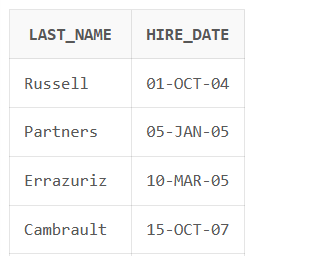
\includegraphics[width=7cm]{Figs/fig_701.png}
  }
}

\lstset{
  basicstyle=\fontsize{10}{12}\selectfont\ttfamily
}

\begin{lstlisting}[language=SQL]
SSELECT 	last_name,
       	TO_CHAR (hire_date, 'DD-MON-YY') hire_date
FROM 	hr.employees
WHERE 	department_id = (
         	SELECT 	department_id
         	FROM 	hr.employees
         	WHERE 	last_name = 'Zlotkey'
   		)
      	AND last_name <> initcap ('Zlotkey');
\end{lstlisting}
\textbf{Output: }
\end{frame}


%--------------------------------------
\newpage
\subsubsection*{Problem 02}
\addcontentsline{toc}{subsection}{Problem 02}
Create a report that displays the employee number, last name, and salary of all employees who earn more than the average salary. Sort the results in order of ascending salary.

\begin{frame}

\AddToShipoutPictureFG*{ % Add figure to foreground of current page
  \put(\LenToUnit{5.5cm},\LenToUnit{13cm}){% Adjust the coordinates as needed
    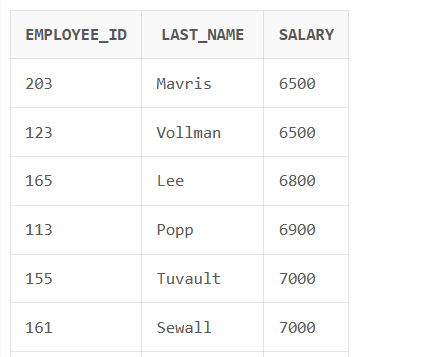
\includegraphics[width=7cm]{Figs/fig_702.png}
  }
}

\lstset{
  basicstyle=\fontsize{10}{12}\selectfont\ttfamily
}

\begin{lstlisting}[language=SQL]
SELECT 	employee_id, last_name, salary
FROM 	hr.employees
WHERE 	salary > (
   			SELECT AVG (salary)
   			FROM 	hr.employees
		)
ORDER BY salary;
\end{lstlisting}
\textbf{Output: }
\end{frame}




%--------------------------------------
\vspace{5cm}
\subsubsection*{Problem 03}
\addcontentsline{toc}{subsection}{Problem 03}
Write a query that displays the employee number and last name of all employees who work in a department with any employee whose last name contains the letter u. Save your SQL statement as lab\_07\_03.sql. Run your query.

\begin{frame}

\AddToShipoutPictureFG*{ % Add figure to foreground of current page
  \put(\LenToUnit{13cm},\LenToUnit{2.3cm}){% Adjust the coordinates as needed
    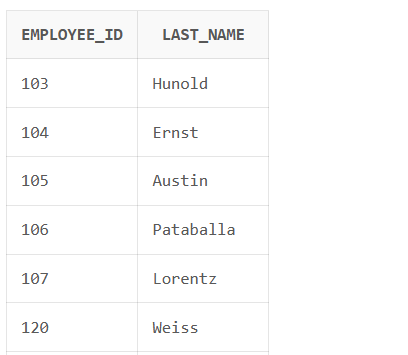
\includegraphics[width=7cm]{Figs/fig_703.png}
  }
}

\lstset{
  basicstyle=\fontsize{10}{12}\selectfont\ttfamily
}

\begin{lstlisting}[language=SQL]
SELECT 	employee_id,
       	last_name
FROM 	hr.employees
WHERE 	department_id IN (
   			SELECT department_id
   			FROM hr.employees
   			WHERE last_name LIKE '%u%'
		);
\end{lstlisting}
\textbf{Output: }
\end{frame}


%--------------------------------------
\newpage
\subsubsection*{Problem 04}
\addcontentsline{toc}{subsection}{Problem 04}
The HR department needs a report that displays the last name, department number, and job ID of all employees whose department location ID is 1700.

\begin{frame}

\AddToShipoutPictureFG*{ % Add figure to foreground of current page
  \put(\LenToUnit{13cm},\LenToUnit{14cm}){% Adjust the coordinates as needed
    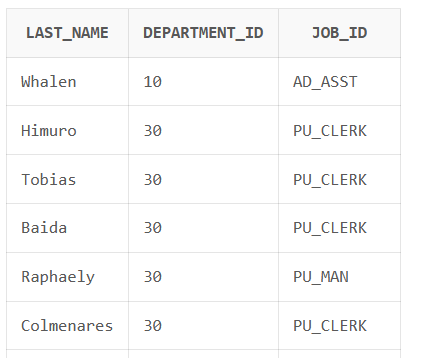
\includegraphics[width=7cm]{Figs/fig_704.png}
  }
}

\lstset{
  basicstyle=\fontsize{10}{12}\selectfont\ttfamily
}

\begin{lstlisting}[language=SQL]
SELECT 	last_name, department_id, job_id
FROM 	hr.employees
WHERE 	department_id IN (
   			SELECT 	department_id
   			FROM 	hr.departments
   			WHERE 	location_id = 1700
		)
ORDER BY department_id;
\end{lstlisting}
\textbf{Output: }
\end{frame}

%--------------------------------------
\vspace{5cm}
Modify the query so that the user is prompted for a location ID. Save this to a file named lab\_07\_04.sql.

\begin{frame}

\AddToShipoutPictureFG*{ % Add figure to foreground of current page
  \put(\LenToUnit{5.5cm},\LenToUnit{4cm}){% Adjust the coordinates as needed
    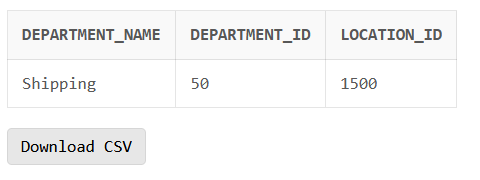
\includegraphics[width=7cm]{Figs/fig_704b.png}
  }
}

\lstset{
  basicstyle=\fontsize{10}{12}\selectfont\ttfamily
}

\begin{lstlisting}[language=SQL]
SELECT 	department_name, department_id, location_id
FROM 	hr.departments
WHERE 	location_id IN (
   			SELECT 	location_id
   			FROM 	hr.locations
   			WHERE 	location_id = 1500
		)
ORDER BY location_id;
\end{lstlisting}
\textbf{Output: }
\end{frame}



%--------------------------------------
\newpage
\subsubsection*{Problem 05}
\addcontentsline{toc}{subsection}{Problem 05}
Create a report for HR that displays the last name and salary of every employee who reports to King.
\begin{frame}

\AddToShipoutPictureFG*{ % Add figure to foreground of current page
  \put(\LenToUnit{5.5cm},\LenToUnit{14cm}){% Adjust the coordinates as needed
    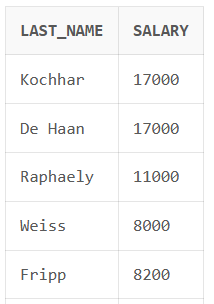
\includegraphics[width=4cm]{Figs/fig_705.png}
  }
}

\lstset{
  basicstyle=\fontsize{10}{12}\selectfont\ttfamily
}

\begin{lstlisting}[language=SQL]
SELECT 	last_name, salary
FROM 	hr.employees
WHERE 	manager_id IN (
   			SELECT 	employee_id
   			FROM 	hr.employees
   			WHERE 	last_name = 'King'
		);
\end{lstlisting}
\textbf{Output: }
\end{frame}



%--------------------------------------
\vspace{5cm}
\subsubsection*{Problem 06}
\addcontentsline{toc}{subsection}{Problem 06}
Create a report for HR that displays the department number, last name, and job ID for every employee in the Executive department.

\begin{frame}

\AddToShipoutPictureFG*{ % Add figure to foreground of current page
  \put(\LenToUnit{5.5cm},\LenToUnit{2.3cm}){% Adjust the coordinates as needed
    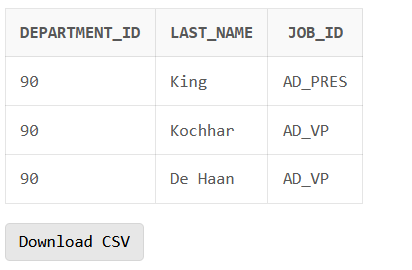
\includegraphics[width=7cm]{Figs/fig_706.png}
  }
}

\lstset{
  basicstyle=\fontsize{10}{12}\selectfont\ttfamily
}

\begin{lstlisting}[language=SQL]
SELECT 	department_id, last_name, job_id
FROM 	hr.employees
WHERE 	department_id = (
   			SELECT 	department_id
   			FROM 	hr.departments
   			WHERE 	department_name = 'Executive'
		);
\end{lstlisting}
\textbf{Output: }
\end{frame}


%--------------------------------------
\newpage
\subsubsection*{Problem 07}
\addcontentsline{toc}{subsection}{Problem 07}
Modify the query in lab\_07\_03.sql to display the employee number, last name, and salary of all employees who earn more than the average salary, and who work in a department with any employee whose last name contains a 'u'. Resave lab\_07\_03.sql as lab\_07\_07.sql. Run the statement in lab\_07\_03.sql.
\begin{frame}

\AddToShipoutPictureFG*{ % Add figure to foreground of current page
  \put(\LenToUnit{5.5cm},\LenToUnit{9cm}){% Adjust the coordinates as needed
    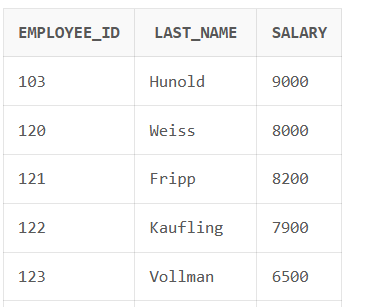
\includegraphics[width=8cm]{Figs/fig_707.png}
  }
}

\lstset{
  basicstyle=\fontsize{10}{12}\selectfont\ttfamily
}

\begin{lstlisting}[language=SQL]
SELECT 	employee_id, last_name, salary
FROM 	hr.employees
WHERE 	salary > (
         	SELECT AVG (salary)
         	FROM 	hr.employees
   		)
    AND department_id IN (
   			SELECT 	department_id
   			FROM 	hr.employees
   			WHERE last_name LIKE '%u%'
	);
\end{lstlisting}
\textbf{Output: }
\end{frame}



	
	
\end{document}